\chapter[Theory and Motivation]{Theory and Motivation}

This chapter aims to provide an overview of the Standard Model of Particle Physics (SM), with a particular focus on the pivotal role played by the Higgs boson. We will briefly introduce the SM and its fundamental particles, as well as the Lagrangian that governs their behavior. Additionally, we will delve into the details of the Higgs boson – its properties, its most frequent production and decay modes, and the Yukawa couplings to the three different fermion families. Finally, we will focus on the decay channels present in our analysis, and explore how a significant discrepancy between the measurements of these decay modes and the SM predictions might lead to new physics beyond the SM.

\section{The Standard Model}

One of the traits that distinguishes humans from other life forms is our sense of curiosity. Since ancient times, we have been trying to explain what happens around us, enabling us to predict and potentially harness the laws of nature. An extraordinary theory that has come very close to achieving this goal is the Standard Model of Particle Physics (SM), one of the most precise theories humanity has ever conceived, and the most successful theory of particle physics to date. The Standard Model is a theory capable of describing three of the four known fundamental forces in the Universe (electromagnetic, weak, and strong force, but not gravity). This is achieved by classifying a set of elementary particles and defining the interactions between them.

More in detail, the SM is a quantum field theory (QFT) defined by an internal local $\text{SU}(3)_{\text{C}}\times \text{SU}(2)_{\text{L}}\times \text{U}(1)_{\text{Y}}$ gauge symmetry. Each elementary particle has its own corresponding field in the theory and is categorized as a fermion or a boson, based on its spin (half-integer-spin particles are fermions, whereas integer-spin particles are bosons). There are twelve fermions organized in three families or generations of four members: a charged lepton (e.g. the electron), a neutral lepton (neutrino), an up-type quark and a down-type quark (in addition, each particle has its own corresponding antiparticle) (see Figure \ref{fig:SM}).

\begin{figure}[!ht]
    \vspace*{-0.0cm}
    \centering
    \setlength{\mylength}{\textwidth}
    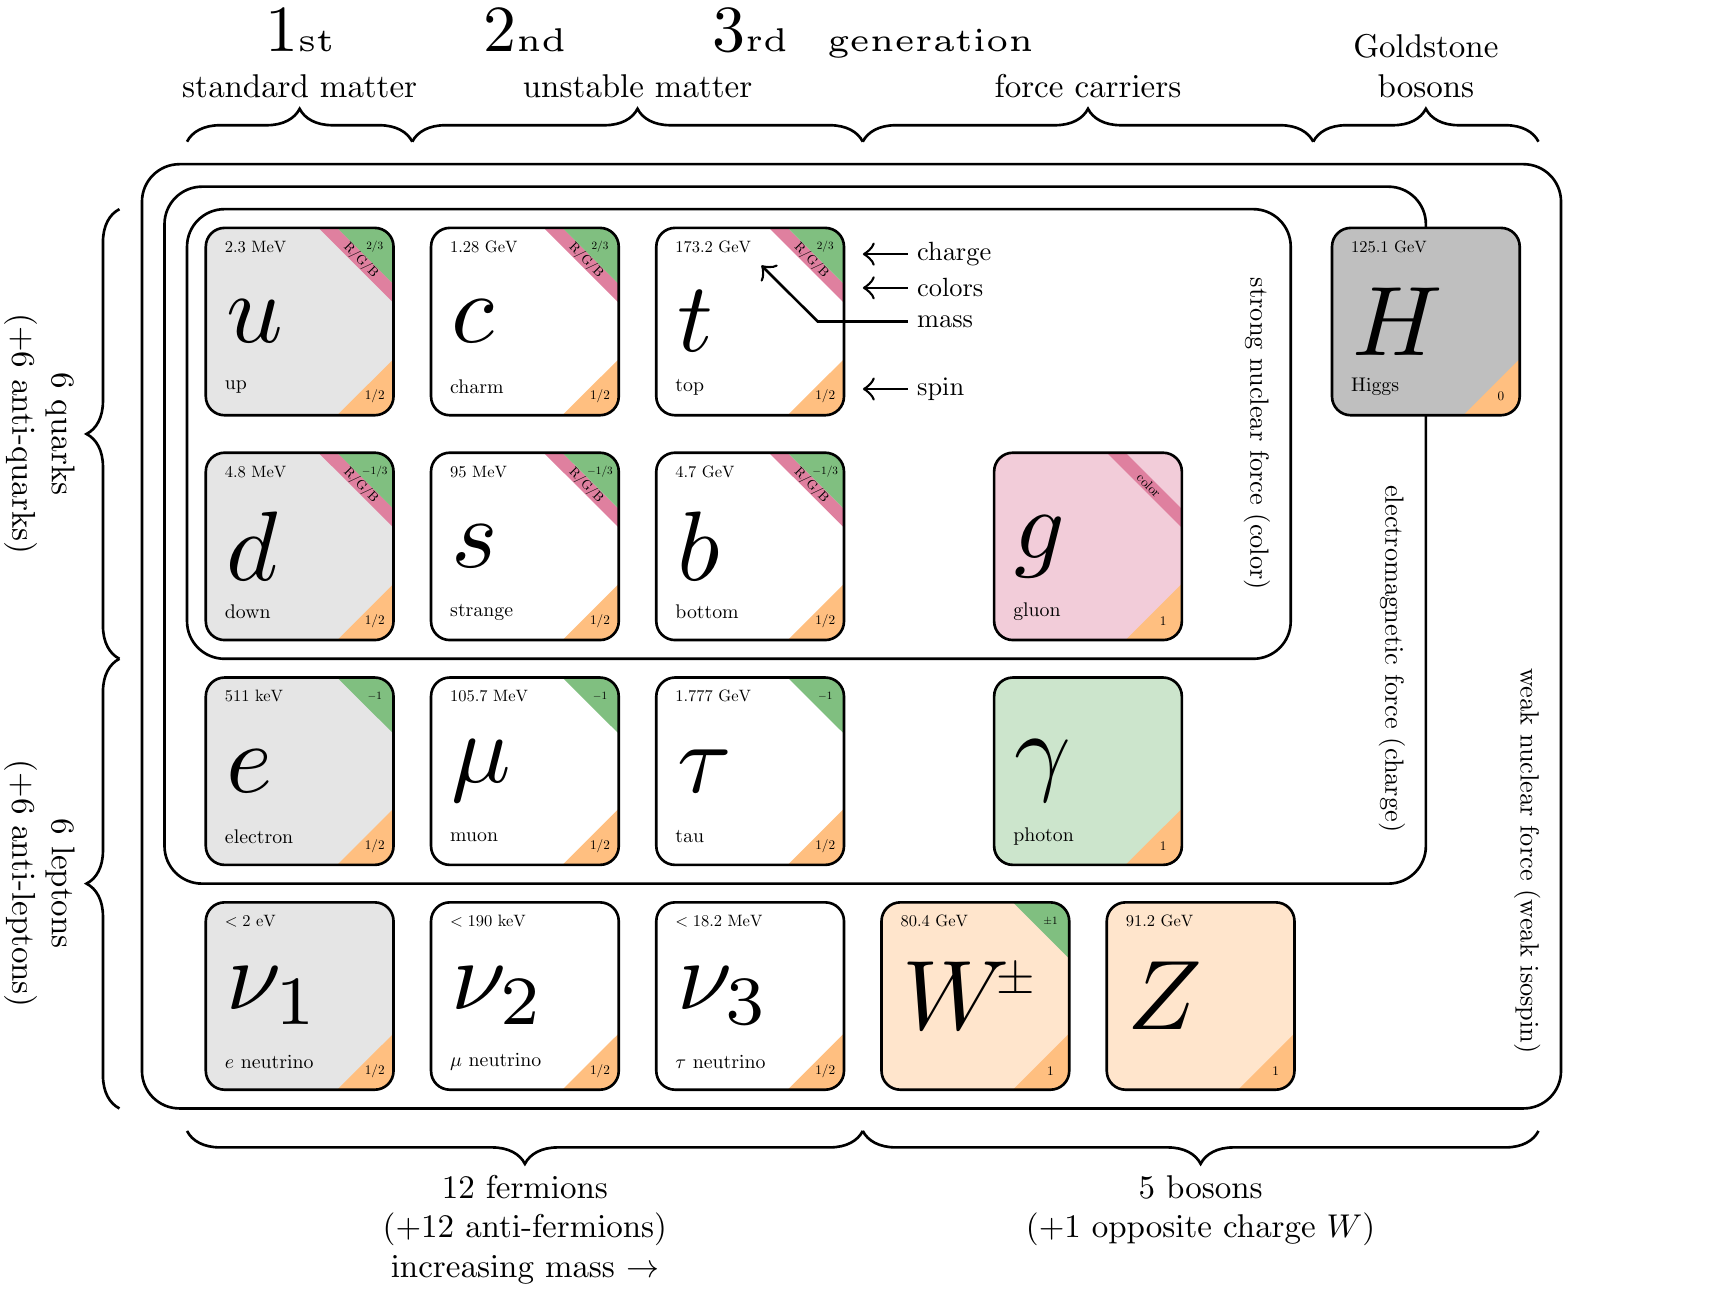
\includegraphics[width=0.8\mylength]{resources/SM.png}
    \vspace*{-0.0cm}
    \caption{Elementary particles of the Standard Model.}
    \label{fig:SM}
    \vspace*{-0.0cm}
\end{figure}

These three factors of the gauge symmetry group give rise to the three fundamental interactions between fermions, which are mediated by gauge bosons. To be precise, each generator of a local invariant gauge group induces a massless gauge boson. The same way that in quantum electrodynamics (QED) the local gauge invariance of the theory under the $\text{U}(1)$ group leads to the existance of a massless, gauge field $A_\mu$ (the photon field), in the SM the process is analogous.

The invariance of the SM under $\text{SU}(3)_{\text{C}}$ postulates the existance of the gluon. More precisely, the eight generators of $\text{SU}(3)_{\text{C}}$ introduce eight gluons that mediate the strong force between particles that possess color charge (quarks). This is known as the quantum chromodynamics (QCD) sector of the standard model.

Similarly, the invariance of the second and third factors $\text{SU}(2)_{\text{L}}\times \text{U}(1)_{\text{Y}}$ indicates the existance of the photon, the $Z^{0}$ and the $W^{\pm}$ bosons. In this case, unlike in QED or QCD, we cannot directly associate the photon to the generator of the hypercharge group $\text{U}(1)_{\text{Y}}$ and the $Z^{0}$, $W^{\pm}$ bosons to the generators of the left weak isospin group $\text{SU}(2)_{\text{L}}$. Instead, the generators of $\text{SU}(2)_{\text{L}}\times \text{U}(1)_{\text{Y}}$ give rise to four intermediate vector bosons ($W_\mu^{1,2,3}$ for $\text{SU}(2)_{\text{L}}$ and $B_\mu$ for $\text{U}(1)_{\text{Y}}$), which are then mixed through the weak mixing angle or Weinberg angle $\theta_{\text{W}}$ to produce the physical $\gamma$ ($A_\mu$), $Z^{0}$, $W^{\pm}$. The physical bosons are then defined as:
\begin{align*}
    W_\mu^{\pm} &= \frac{1}{\sqrt{2}}(W_\mu^{1}\mp iW_\mu^{2})\\
    \begin{pmatrix}
        A_\mu \\
        Z^{0}_\mu
    \end{pmatrix}
    &=
    \begin{pmatrix}
        \cos{\theta_{\text{W}}} & \sin{\theta_{\text{W}}} \\
        -\sin{\theta_{\text{W}}} & \cos{\theta_{\text{W}}}
    \end{pmatrix}
    \begin{pmatrix}
        B_\mu \\
        W^{3}_\mu
    \end{pmatrix}
\end{align*}
By definition of the groups $\text{SU}(2)_{\text{L}}$ and $\text{U}(1)_{\text{Y}}$, the field $W_\mu^{1,2,3}$ couples only to left-handed (negative helicity) particles, whereas the hypercharge field $B_\mu$ couples to both left and right components with the same strength. Therefore, the intermediate boson mixing implies that $W^{\pm}$ only couple to left-handed particles, but $Z^{0}$ couples to both left and right-handed particles with different strengths, inducing parity violation (although not maximal).

All gauge bosons that arise from the generators of gauge invariant groups are to be massless, or else the principle of local gauge invariance is spoiled and the theory becomes unrenormalizable. But this is in contradiction with experiments, from where we know that the $Z^{0}$, $W^{\pm}$ bosons are in fact massive. This breaking of gauge invariance when giving a mass to a particle is not restricted only to gauge bosons, but also happens for fermions. In the SM, to be able to have massive fields, all particles obtain their masses using spontanoeus symmetry breaking (SSB) via the Higgs mechanism.

Spontaneous symmetry breaking is a fundamental principle of QFT to explain how gauge bosons (and, in general, massive particles) can acquire non-vanishing mass. This process describes systems where the Lagrangian obeys symmetries, but the lowest-energy vacuum solutions do not exhibit the same symmetries. In the case of the Higgs mechanism, it relies on the existance of a $\text{SU}(2)$ doublet complex scalar field $\phi$ with hypercharge $Y = +1$, which can be written as 
\begin{equation*}
    \phi=
    \begin{pmatrix}
        \phi^{+} \\
        \phi^{0}
    \end{pmatrix}
\end{equation*}
with $(\phi^{+})^{*}=\phi^{-}$ and $(\phi^{0})^{*}=\phi^{0}$, with Lagrangian density $\mathcal{L}=\abs{D_{\mu}\phi}^2 - V(\phi)$ and potential $V(\phi) = \mu^2\phi^\dag\phi+\lambda(\phi^\dag\phi)^2$, where $D_\mu$ is the covariant derivative determined by $\text{SU}(2)_{\text{L}}\times \text{U}(1)_{\text{Y}}$. When expanding the field $\phi$ around a minimum of the potential $V$, one finds out that there are infinitely many values $\phi$ that minimize the potential. Suppose one expands $\phi$ around
\begin{equation*}
    \phi_{0}=\frac{1}{\sqrt{2}}
    \begin{pmatrix}
        0 \\
        v
    \end{pmatrix},\quad \text{so}\quad
    \phi(x)=\frac{1}{\sqrt{2}}
    \begin{pmatrix}
        0 \\
        v + h(x)
    \end{pmatrix}.
\end{equation*}
Deciding to expand the field around a chosen minimum $\phi_{0}$ spontaneously breaks the $\text{SU}(2)_{\text{L}}\times \text{U}(1)_{\text{Y}}$ symmetry, which in turn generates mass terms for the weak bosons in the Lagrangian. To convince oneself of the last implication it suffices to expand the $\abs{D_{\mu}\phi}^2$ term around the chosen vacuum expectation value $v$, which will produce terms of the form $M_{W}^2W_\mu^{+}W^{-\mu}$ and $M_{Z}^2Z_\mu^{0}Z^{0\mu}$ in the Lagrangian density. This scalar field is called the Higgs field.

With that, the Standard Model of particle physics is governed by the following Lagrangian density:
\begin{equation}
\begin{aligned}
    \mathcal{L}_{\text{SM}} &= -\frac{1}{4}G_{\mu\nu}^{a}G^{a\mu\nu} -\frac{1}{4}W_{\mu\nu}^{i}W^{i\mu\nu} -\frac{1}{4}B_{\mu\nu}B^{\mu\nu} \label{eq:L_SM}\\
    &+ \abs{D_\mu\phi}^2 - \mu^2\phi^\dag\phi - \lambda(\phi^\dag\phi)^2 \\
    &+ i\left[\bar{L}\slashed{D} L + \bar{e}\slashed{D} e + \bar{Q}\slashed{D} Q + \bar{u}\slashed{D} u + \bar{d}\slashed{D} d\right] \\
    & -\left[Y_{e}\bar{L}\phi e + Y_u\bar{Q}\phi^{c} u + Y_d\bar{Q}\phi d + \text{h.c.}\right]
\end{aligned}
\end{equation}
The used notation is the following: $\phi$, $Q$, $u$, $d$, $L$, $e$ are the SM Higgs, quarks and lepton fields. The left-handed doublets are denoted by capital letters as
\begin{equation*}
    Q_{i} = 
    \begin{pmatrix}
    u_{L}^{i}\\
    d_{L}^{i}
    \end{pmatrix}
    \text{ for quarks, and } L_{\alpha} = 
    \begin{pmatrix}
    \nu_{L}^{\alpha}\\
    e_{L}^{\alpha}
    \end{pmatrix}\text{for leptons,}
\end{equation*}
whereas for the right-handed singlets lowercase letters are used. We use the usual covariant derivative defined as
\begin{equation*}
    D_\mu = \partial_\mu + ig_{s}T^{a}G_\mu^{a} + ig\frac{\sigma^{i}}{2}W_\mu^{i} + ig'YB_\mu
\end{equation*}
and where $T^{a}$ and $\sigma^{i}$ are the generators of SU(3) and SU(2), respectively. 

The first line in Equation \eqref{eq:L_SM} describes the kinetic energies and interactions of the gauge boson fields. The field strength tensors associated to $G_\mu^{a}$ (gluons), $W_\mu^{i}$ and $B_\mu$ ($W^{\pm}, Z^{0}, \gamma$) are defined by
\begin{align*}
    G_{\mu\nu}^{a} &= \partial_\mu G_\nu^{a} - \partial_\nu G_\mu^{a} - g_{s} f^{abc}G_\mu^{b}G_\nu^{c}\\
    W_{\mu\nu}^{i} &= \partial_\mu W_\nu^{i} - \partial_\nu W_\mu^{i} - g \epsilon^{ijk}W_\mu^{j}W_\nu^{k}\\
    B_{\mu\nu} &= \partial_\mu B_\nu - \partial_\nu B_\mu
\end{align*}
where $f^{abc}$ and $\epsilon^{ijk}$ are the group structure constants of SU(3) and SU(2), respectively (the strength tensor of the hypercharge field $B_\mu$ does not have this extra term since U(1) is abelian). This is why gluons and electroweak bosons are self-interacting.

The second line in Equation \eqref{eq:L_SM} describes the Higgs field and generates the masses of the weak gauge bosons $W^{\pm}$, $Z^{0}$ and of the Higgs boson. In particular, the term $\abs{D_{\mu}\phi}^2$ generates all interactions between the gauge bosons and the Higgs field.

The third line in Equation \eqref{eq:L_SM} is responsible for fermion kinetic energies as well as their interactions with all bosons (gluons and eletroweak bosons). We have five terms: left-handed lepton doublets, right-handed lepton singlets (only charged leptons since right-handed neutrinos do not couple in the SM), left-handed quark doublets, right-handed up-type quark singlets and right-handed down-type quark singlets. The covariant derivative terms relative to each group apply only to these fermions that transform under that group. For instance, the first term would expand as
\begin{equation*}
    i\bar{L}\slashed{D} L = i\bar{L}\gamma^{\mu}D_\mu L = i
    \begin{pmatrix}
        \bar{\nu}_{L}^{\alpha} & \bar{e}_{L}^{\alpha}
    \end{pmatrix}
    \gamma^{\mu}\left(\partial_\mu + ig\frac{\sigma^{i}}{2}W_\mu^{i} + ig'YB_\mu\right)
    \begin{pmatrix}
        \nu_{L}^{\alpha}\\
        e_{L}^{\alpha}
    \end{pmatrix},
\end{equation*}
since the leptons do not carry color charge, but the fourth term would expand as
\begin{equation*}
    i\bar{u}\slashed{D} u = i\bar{u}\gamma^{\mu}D_\mu u = i \bar{u}_{R}^{i}
    \gamma^{\mu}\left(\partial_\mu + ig_{s}T^{a}G_\mu^{a} + ig'YB_\mu\right) u_{R}^{i},
\end{equation*}
because the right-handed quark is a singlet under SU(2)$_{\text{L}}$.

Finally, the couplings between the Higgs boson and the fermions, and in turn fermion masses, are generated by the fourth line in Equation \eqref{eq:L_SM}. These terms are gauge invariant, but give rise to fermion masses. For example, for the leptons and taking the Higgs field expansion around $\phi_0$, the first term will expand as
\begin{equation*}
    Y_{e}\bar{L}\phi e = \frac{Y_e^{\alpha\beta}}{\sqrt{2}}
    \begin{pmatrix}
        \bar{\nu}_{L}^{\alpha} & \bar{e}_{L}^{\alpha}
    \end{pmatrix}
    \begin{pmatrix}
        0\\
        v + h(x)
    \end{pmatrix}
    e_{R}^{\beta} = \frac{Y_e^{\alpha\beta}}{\sqrt{2}}\left[v + h(x)\right] \bar{e}_{L}^{\alpha}e_{R}^{\beta}
\end{equation*}
which in addition to its hermitian conjugate will ultimately yield the term
\begin{equation*}
    \frac{Y_e^{\alpha\beta}}{\sqrt{2}} v \left[\bar{e}_{L}^{\alpha}e_{R}^{\beta} + \bar{e}_{R}^{\alpha}e_{L}^{\beta}\right] = \frac{Y_e^{\alpha\beta}v}{\sqrt{2}} \bar{e}^{\alpha}e^{\beta}
\end{equation*}
after spontaneous symmetry breaking. One can easily identify the mass of the three charged leptons as
\begin{equation*}
    m_{e} = \frac{Y_e^{ee} v}{\sqrt{2}},\quad m_{\mu} = \frac{Y_e^{\mu\mu} v}{\sqrt{2}}\quad\text{and}\quad m_{\tau} = \frac{Y_e^{\tau\tau} v}{\sqrt{2}}.
\end{equation*}
To generate mass terms for up-type like quarks the Yukawa term involves the charge conjugate of the Higgs doublet (as in the second term of the fourth line in Equation \eqref{eq:L_SM}).

The Standard Model Lagrangian \eqref{eq:L_SM} induces the interactions between all particles present in the theory. These interactions can be seen as Feynman diagram vertices, shown in Figure \ref{fig:SM_vertices}.

\todo{Explain SM feynman diagrams}

\begin{figure}[!ht]
    \captionsetup[subfigure]{labelformat=empty}
    \vspace*{-0.2cm}
    \centering
    \setlength{\mylength}{\textwidth}
    \begin{subfigure}[t]{0.33\mylength}
            \centering
            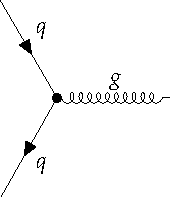
\includegraphics[height=0.20\mylength]{resources/SM_vertices/v1.pdf}
            \setlength{\unitlength}{0.25\mylength}
            %\caption{\footnotesize (a)}
    \end{subfigure}%
    \begin{subfigure}[t]{0.33\mylength}
            \centering
            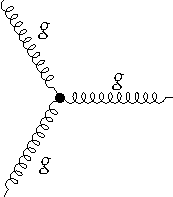
\includegraphics[height=0.20\mylength]{resources/SM_vertices/v2.pdf}
            \setlength{\unitlength}{0.25\mylength}
            %\caption{\footnotesize (b)}
    \end{subfigure}%
    \begin{subfigure}[t]{0.33\mylength}
            \centering
            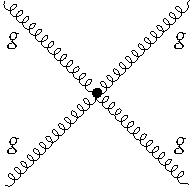
\includegraphics[height=0.20\mylength]{resources/SM_vertices/v3.pdf}
            \setlength{\unitlength}{0.25\mylength}
            %\caption{\footnotesize (c)}
    \end{subfigure}%\begin{subfigure}[t]{0.33\mylength}\baselineskip    
    \vskip\baselineskip
    \vspace*{-0.1cm}
    \begin{subfigure}[t]{0.33\mylength}
            \centering
            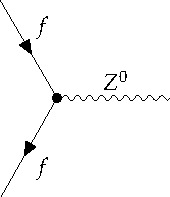
\includegraphics[height=0.20\mylength]{resources/SM_vertices/v4.pdf}
            \setlength{\unitlength}{0.25\mylength}
            %\caption{\footnotesize (d)}
    \end{subfigure}%\begin{subfigure}[t]{0.33\mylength}
    \begin{subfigure}[t]{0.33\mylength}
            \centering
            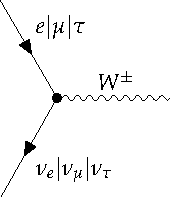
\includegraphics[height=0.20\mylength]{resources/SM_vertices/v5.pdf}
            \setlength{\unitlength}{0.25\mylength}
            %\caption{\footnotesize (e)}
    \end{subfigure}%\begin{subfigure}[t]{0.33\mylength}
    \begin{subfigure}[t]{0.33\mylength}
            \centering
            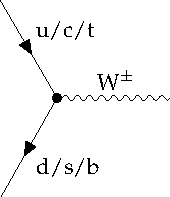
\includegraphics[height=0.20\mylength]{resources/SM_vertices/v6.pdf}
            \setlength{\unitlength}{0.25\mylength}
            %\caption{\footnotesize (f)}
    \end{subfigure}%
    \vskip\baselineskip
    \vspace*{-0.1cm}
    \begin{subfigure}[t]{0.33\mylength}
            \centering
            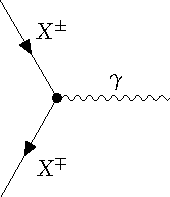
\includegraphics[height=0.20\mylength]{resources/SM_vertices/v7.pdf}
            \setlength{\unitlength}{0.25\mylength}
            %\caption{\footnotesize (g)}
    \end{subfigure}%\begin{subfigure}[t]{0.33\mylength}
    \begin{subfigure}[t]{0.33\mylength}
            \centering
            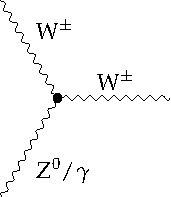
\includegraphics[height=0.20\mylength]{resources/SM_vertices/v8.pdf}
            \setlength{\unitlength}{0.25\mylength}
            %\caption{\footnotesize (h)}
    \end{subfigure}%\begin{subfigure}[t]{0.33\mylength}
    \begin{subfigure}[t]{0.33\mylength}
            \centering
            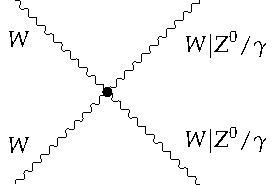
\includegraphics[height=0.20\mylength]{resources/SM_vertices/v9.pdf}
            \setlength{\unitlength}{0.25\mylength}
            %\caption{\footnotesize (i)}
    \end{subfigure}%
    \vskip\baselineskip
    \vspace*{-0.1cm}
    \begin{subfigure}[t]{0.33\mylength}
            \centering
            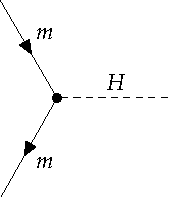
\includegraphics[height=0.20\mylength]{resources/SM_vertices/v10.pdf}
            \setlength{\unitlength}{0.25\mylength}
            %\caption{\footnotesize (j)}
    \end{subfigure}%\begin{subfigure}[t]{0.33\mylength}
    \begin{subfigure}[t]{0.33\mylength}
            \centering
            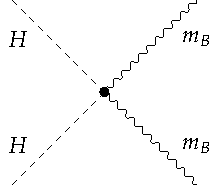
\includegraphics[height=0.20\mylength]{resources/SM_vertices/v11.pdf}
            \setlength{\unitlength}{0.25\mylength}
            %\caption{\footnotesize (k)}
    \end{subfigure}%\begin{subfigure}[t]{0.33\mylength}
    \vspace*{-0.0cm}
    \caption{All possible interactions in the Standard Model, represented by Feynman diagrams. $q$ is any quark, $g$ is (any) gluon, $X^{\pm}$ is any charged particle, $\gamma$ is a photon, $f$ is any fermion, $m$ is any massive particle (with the possible exception of the neutrinos), $m_{B}$ is any boson with mass. In diagrams with multiple particle labels separated by / one particle label is chosen. In diagrams with particle labels separated by | the labels must be chosen in the same order. For example, in the four boson electroweak case the valid diagrams are $WWWW$, $WWZZ$, $WW\gamma\gamma$ and $WWZ\gamma$. The conjugate of each listed vertex (reversing the direction of arrows) is also allowed.}
    \label{fig:SM_vertices}
    \vspace*{-0.0cm}
\end{figure}

The Standard Model has proven to predict numerous measurements with exceptional precision, yet the theory does not explain why the masses of all particles are given by the values we measure. In fact, aside from the mass of the photon, which is protected by the unbroken U(1) gauge symmetry of QED, the SM does not predict any other mass value. All fermion masses (or equivalently the Yukawa couplings) are free parameters of the theory.

While this theory has been remarkably successful, it cannot serve as the final theory of nature, as numerous unresolved puzzles persist. Many cosmological observations remain unaccounted for by the SM, i.e., the baryon-antibaryon asymmetry, the behaviour of gravity as described by General Relativity, the accelerated expansion of the Universe — potentially described by dark energy — and the absence of a suitable candidate for dark matter. Furthermore, the SM fails to explain the non-vanishing mass of the neutrinos as a consequence of neutrino flavour oscillation. In pursuit of a superior theory capable of encompassing the SM as well as these (and many other) discrepancies, the physics community is thoroughly trying to ``break'' the Standard Model to unveil hints towards an ultimate theory.

\section{The Higgs boson}

In 1964, Peter Higgs, along with five other theoretical physicists, proposed the Higgs mechanism to explain how certain particles (fermions and weak bosons) might acquire mass in local gauge theories \cite{Higgs:1964pj,Englert:1964et,Guralnik:1964eu}. If these ideas were correct, a spin-0 particle (namely the Higgs boson) should exist and possess some well-defined properties. Nearly 50 years later, on the 4\textsuperscript{th} of July of 2012, a scalar particle consistent with the Higgs boson was discovered at the LHC by the CMS and ATLAS collaborations \cite{CMS:2012qbp,ATLAS:2012yve}.

The Higgs boson is a weak isospin SU(2)$_{\text{L}}$ doublet, massive scalar boson, this is, a particle with spin 0. Table \ref{tab:higgs_properties} summarizes the SM predicted properties \cite{Djouadi:2005gi,LHCHiggsCrossSectionWorkingGroup:2016ypw} as well as the measured properties of the Higgs boson from the Particle Data Group (PDG) \cite{PDG}.

\begin{table}[ht]
    \centering
    \begin{tabular}{|l|l|l|}
        \hline
        \cellcolor{lightgray}Property & \cellcolor{lightgray}SM prediction & \cellcolor{lightgray}Mesasured value \\ \hline
        Mass                & $m \lesssim 700 \;\; \text{GeV}$ & $m = 125.25 \pm 0.17 \;\; \text{GeV}$             \\
        Spin                &  $J=0$ & $J=0$                                             \\
        Electric charge     & $q=0$  & $q=0$                                             \\
        Full width          & $\Gamma = 4.12 \pm 0.06 \;\;  \text{MeV}$  & $\Gamma = 3.2^{+2.8}_{-2.2} \;\;  \text{MeV}$     \\
        Lifetime            & $\tau = (1.60 \pm 0.02) \times 10^{-22} \;\;  \text{s}$  & $\tau = 2.1^{+4.5}_{-1.0} \times 10^{-22} \;\;  \text{s}$   \\ \hline
    \end{tabular}
    \caption{Properties of the Higgs boson. The SM prediction for the full width and the lifetime depend on the Higgs mass, which is assumed to be $m = 125.25$ GeV.}
    \label{tab:higgs_properties}
\end{table}

As stated previously, the SM does not predict the mass of any particle (except for the photon), including the mass of the Higgs boson. Nevertheless, some theoretical arguments, such as radiative corrections and unitarity considerations, enabled theorists to establish upper bounds on the Higgs mass \cite{Djouadi:2005gi}.

To understand the production and decay modes of the Higgs boson, it's important to recall that the Higgs boson couples to all the other particles of the SM (it couples to the gauge bosons via the $\abs{D_{\mu}\phi}^2$ term in Higgs part of Equation \eqref{eq:L_SM} and to fermions via the Yukawa couplings in the last line of Equation \eqref{eq:L_SM}), as well as to itself. By expanding the terms in the Lagrangian, it can be seen that the coupling between the Higgs boson and any massive particle is directly proportional to the particle's rest mass.

Collecting the relevant Feynman vertices one can get the dominant production modes for the Higgs boson, as seen in Figure \ref{fig:Higgs_production}. Since the heavier the particle, the stronger its Higgs coupling constant is, we see that in most cases particles present in the vertex where the Higgs boson is produced are very heavy (top and bottom quarks and massive gauge bosons).

\todo{Talk about Higgs production at LHC}

\begin{figure}[!ht]
    \captionsetup[subfigure]{labelformat=empty}
    \vspace*{-0.2cm}
    \centering
    \setlength{\mylength}{\textwidth}
    \begin{subfigure}[t]{0.33\mylength}
            \centering
            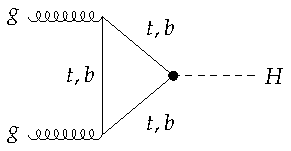
\includegraphics[height=0.17\mylength]{resources/H_production_diagrams/v1.pdf}
            \setlength{\unitlength}{0.25\mylength}
            \caption{\footnotesize (a)}
    \end{subfigure}%
    \begin{subfigure}[t]{0.33\mylength}
            \centering
            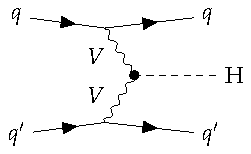
\includegraphics[height=0.17\mylength]{resources/H_production_diagrams/v2.pdf}
            \setlength{\unitlength}{0.25\mylength}
            \caption{\footnotesize (b)}
    \end{subfigure}%
    \begin{subfigure}[t]{0.33\mylength}
            \centering
            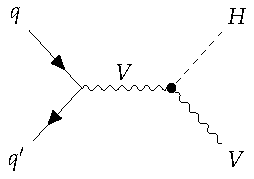
\includegraphics[height=0.20\mylength]{resources/H_production_diagrams/v3.pdf}
            \setlength{\unitlength}{0.25\mylength}
            \caption{\footnotesize (c)}
    \end{subfigure}%\begin{subfigure}[t]{0.33\mylength}\baselineskip    
    \vskip\baselineskip
    \vspace*{-0.1cm}
    \begin{subfigure}[t]{0.33\mylength}
            \centering
            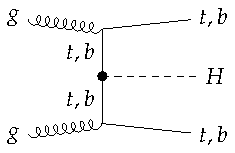
\includegraphics[height=0.17\mylength]{resources/H_production_diagrams/v4.pdf}
            \setlength{\unitlength}{0.25\mylength}
            \caption{\footnotesize (d)}
    \end{subfigure}%\begin{subfigure}[t]{0.33\mylength}
    \begin{subfigure}[t]{0.33\mylength}
            \centering
            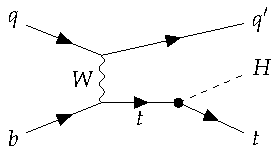
\includegraphics[height=0.17\mylength]{resources/H_production_diagrams/v5.pdf}
            \setlength{\unitlength}{0.25\mylength}
            \caption{\footnotesize (e)}
    \end{subfigure}%\begin{subfigure}[t]{0.33\mylength}
    \begin{subfigure}[t]{0.33\mylength}
            \centering
            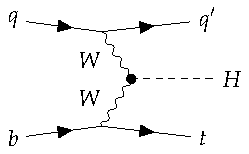
\includegraphics[height=0.17\mylength]{resources/H_production_diagrams/v6.pdf}
            \setlength{\unitlength}{0.25\mylength}
            \caption{\footnotesize (f)}
    \end{subfigure}%
    \vspace*{-0.0cm}
    \caption{Higgs boson production in (a) gluon-gluon fusion (ggH), (b) vector boson fusion (VBF), (c) associated production with a $W$ or $Z$ (V) boson (VH), (d) associated production with a top or bottom quark pair (ttH or bbH), (e, f) associated production with a single top quark (tH).}
    \label{fig:Higgs_production}
    \vspace*{-0.0cm}
\end{figure}

\todo{Higgs production rates SM/measured}

To compare the different production cross sections with the SM it is useful to define the \textit{signal strength} $\mu$ as the measured producion cross section times branching fraction divided by the expected SM value. According to the SM, the total Higgs boson cross section at a center of mass energy of $\sqrt{s} = 13$ TeV is $\sigma = 55400 \pm 2600$ fb \cite{LHCHiggsCrossSectionWorkingGroup:2016ypw}, with around 87\% coming from gluon fusion. The predicted and measured cross section of the Higgs boson at $\sqrt{s} = 13$ TeV from different production modes are shown in Table \ref{tab:Higgs_production}.

\comm{I am not sure if I can compute the measured $\sigma$ like $\sigma_{measured} = \sigma_{SM}\mu$, because there is also the cross section. I have computed, both for the production cross sections and decay branching rations, the measurements like $v_{measured} = v_{SM}\mu$, where $v$ is either the production cross section or the decay branching ratio. Is this correct?}

\begin{table}[ht]
    \centering
    \begin{tabular}{|l|c|c|c|}
        \hline
        \cellcolor{lightgray}Production mode & \cellcolor{lightgray} SM $\sigma$ [fb] & \cellcolor{lightgray} Measured $\sigma$ [fb] & \cellcolor{lightgray} Measured $\mu$ \\ \hline
        ggH                         & $48400 \pm 2400$          & $47000 \pm 4500$          & $0.97 \pm 0.08$           \\
        VBF                         & $3770 \pm 80$             & $3020 \pm 870$            & $0.80 \pm 0.12$    \\
        WH                          & $1365  \pm 28$            & $2030  \pm 360$           & $1.49 \pm 0.26$     \\
        %W$^+$H ($W^+\to l^+\nu$)    & $3\times(93.7  \pm 1.8)$  & $0.0  \pm 0.0$        \\
        %W$^+$H                      & $835  \pm 17$             & $0.0  \pm 0.0$        \\
        %W$^-$H ($W^-\to l^-\nu$)    & $3\times(59.4  \pm 1.2)$  & $0.0  \pm 0.0$        \\
        %W$^-$H                      & $530  \pm 11$             & $0.0  \pm 0.0$        \\
        Z$^0$H                      & $879  \pm 36$             & $1130  \pm 220$           & $1.29 \pm 0.24$    \\
        %Z$^0$H ($Z^0\to l^-l^+$)    & $3\times(29.7  \pm 1.2)$  & $0.0  \pm 0.0$        \\
        %ggZ$^0$H ($Z^0\to l^-l^+$)  & $3\times(93.7  \pm 1.8)$  & $0.0  \pm 0.0$        \\
        %Z$^0$H ($Z^0\to \nu\bar{\nu}$)& $3\times(177  \pm 7)$  & $0.0  \pm 0.0$        \\
        %ggZ$^0$H ($Z^0\to \nu\nu$)  & $3\times(93.7  \pm 1.8)$  & $0.0  \pm 0.0$        \\
        ttH +tH                     & $582  \pm 61$             & $660  \pm 130$             & $1.13 \pm 0.18$    \\
        %ttH                        & $505  \pm 50$            & $0.0  \pm 0.0$        \\
        bbH                         & $480  \pm 120$            & Not measured       & Not measured \\ \hline
        %tH + tbarH (s and t channels)                  & $77  \pm 12$            & $0.0  \pm 0.0$        \\ \hline
    \end{tabular}
    \caption{Cross section of the Higgs boson's most frequent production modes at $\sqrt{s} = 13$ TeV. SM values from \cite{LHCHiggsCrossSectionWorkingGroup:2016ypw}, measured values from \cite{CMS:2022dwd}.}
    \label{tab:Higgs_production}
\end{table}

Once the Higgs boson is produced it decays almost instantly into lighter particles. According to the SM Yukawa couplings of the Higgs field to the fermions, at the first loop order, the Higgs boson predominantly decays to the most massive particles that are kinematically accessible. Despite than, there are certain decay modes where the Higgs boson decays into massless particles (to a pair of gluons or photons), for the first loop contributions are not negligible. The most relevant Feynman diagrams of the Higgs boson decay are shown in Figure \ref{fig:Higgs_decays}. Table \ref{tab:Higgs_decays} shows the most frequent decay channels for the Higgs boson, comparing the SM predicted value to the measured value for the different channels.

\todo{Higgs decays. Why no measurement H->gg.}

\begin{figure}[!ht]
    \captionsetup[subfigure]{labelformat=empty}
    \vspace*{-0.2cm}
    \centering
    \setlength{\mylength}{\textwidth}
    \begin{subfigure}[t]{0.5\mylength}
            \centering
            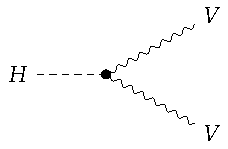
\includegraphics[height=0.17\mylength]{resources/H_decay_diagrams/v1.pdf}
            \setlength{\unitlength}{0.25\mylength}
            \caption{\footnotesize (a)}
    \end{subfigure}%
    \begin{subfigure}[t]{0.5\mylength}
            \centering
            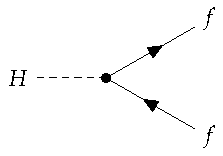
\includegraphics[height=0.17\mylength]{resources/H_decay_diagrams/v2.pdf}
            \setlength{\unitlength}{0.25\mylength}
            \caption{\footnotesize (b)}
    \end{subfigure}%
    \vskip\baselineskip
    \vspace*{-0.1cm}
    \begin{subfigure}[t]{0.5\mylength}
            \centering
            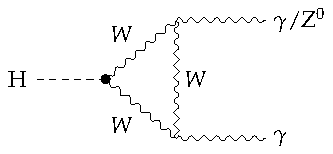
\includegraphics[height=0.17\mylength]{resources/H_decay_diagrams/v3.pdf}
            \setlength{\unitlength}{0.25\mylength}
            \caption{\footnotesize (c)}
    \end{subfigure}%\begin{subfigure}[t]{0.5\mylength}
    \begin{subfigure}[t]{0.5\mylength}
            \centering
            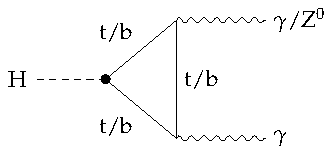
\includegraphics[height=0.17\mylength]{resources/H_decay_diagrams/v4.pdf}
            \setlength{\unitlength}{0.25\mylength}
            \caption{\footnotesize (d)}
    \end{subfigure}%\begin{subfigure}[t]{0.5\mylength}
    \vspace*{-0.0cm}
    \caption{Higgs boson decays into (a) heavy vector boson pairs ($V$ is $Z^{0}/W^{\pm}$), (b) fermion-antifermion pairs, and (c, d) photon pairs or $Z^0\gamma$. Note that $\text{H}\protect\decaysto gg$ is forbidden at tree level, but its non-negligoble branching fraction comes from a heavy quark loop like in (b).}
    \label{fig:Higgs_decays}
    \vspace*{-0.0cm}
\end{figure}

\begin{table}[!ht]
    \centering
    \begin{tabular}{|l|c|c|c|}
        \hline
        \cellcolor{lightgray}Decay channel & \cellcolor{lightgray} SM $\mathcal{B}$ (\%) & \cellcolor{lightgray} Measured $\mathcal{B}$ (\%) & \cellcolor{lightgray} Measured $\mu$ \\ \hline
        $\text{H}\decaysto b\bar{b}$     & $57.8 \pm 0.7$        & $60 \pm 12$         & $1.04 \pm 0.20$ \cite{CMS:2018nsn}  \\
        $\text{H}\decaysto WW^*$         & $21.8 \pm 0.3$        & $20.7 \pm 2.1$      & $0.95 \pm 0.09$ \cite{CMS:2022uhn}  \\
        $\text{H}\decaysto gg$           & $8.2 \pm 0.4$         & Not measured (QCD bkg)    &   \\
        $\text{H}\decaysto \tau^+\tau^-$ & $6.23 \pm 0.10$       & $6.1 \pm 1.1$       & $0.98 \pm 0.18$ \cite{CMS:2017zyp}  \\
        $\text{H}\decaysto c\bar{c}$     & $2.87 \pm 0.16$       & $<40$               & $<14$ \cite{CMS:2022psv}            \\
        $\text{H}\decaysto ZZ^*$         & $2.68 \pm 0.04$       & $2.6 \pm 0.3$       & $0.97 \pm 0.12$ \cite{CMS:2022dwd}  \\
        $\text{H}\decaysto \gamma\gamma$ & $0.227 \pm 0.005$     & $0.254 \pm 0.021$   & $1.12 \pm 0.09$ \cite{CMS:2021kom}  \\
        $\text{H}\decaysto Z\gamma$      & $0.155 \pm 0.009$     & $0.37 \pm 0.14$     & $2.4 \pm 0.9$ \cite{CMS:2022ahq}    \\
        $\text{H}\decaysto \mu^+\mu^-$   & $0.0216 \pm 0.0004$   & $0.026 \pm 0.009$   & $1.19 \pm 0.43$ \cite{CMS:2020xwi}  \\ \hline
    \end{tabular}
    \caption{Most frequent decay modes of the Higgs boson.}
    \label{tab:Higgs_decays}
\end{table}

\section{Searching of a model beyond the SM}

If the Standard Model is right, the coupling between the Higgs boson and every massive fermion is proportional to the fermion's mass. That is why we can create the plot in Figure \ref{fig:Yukawa_couplings}, which according to the SM should follow a straight line. So far the measured values for the massive weak bosons, the third generation of fermions (top and bottom quarks and the tau lepton) and the second generation lepton (the muon) are in perfect agreement with the Standard Model predictions, as seen in Figure \ref{fig:Yukawa_couplings}. \todo{cite the source of this plot}.

\todo{Clean and redo plot of the couplings to the different families}

\begin{figure}[!ht]
    \vspace*{-0.0cm}
    \centering
    \setlength{\mylength}{\textwidth}
    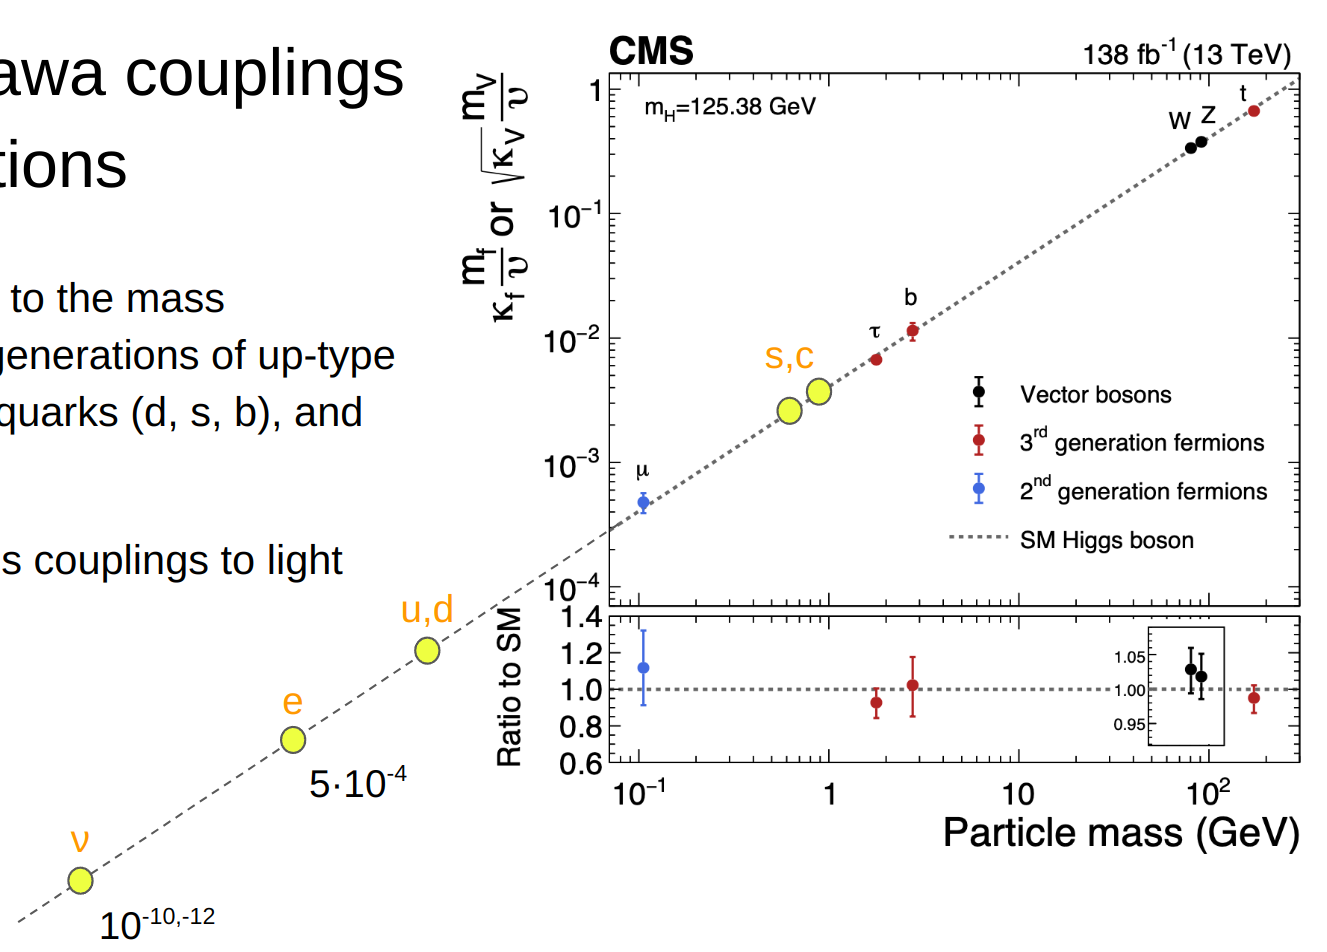
\includegraphics[width=0.80\mylength]{resources/Yukawa_couplings.png}
    \vspace*{-0.0cm}
    \caption{Yukawa couplings.}
    \label{fig:Yukawa_couplings}
    \vspace*{-0.0cm}
\end{figure}

It is interesting to explore the SM with regard to lighter fermions, specifically the second-generation strange and charm quarks, as well as all first-generation fermions, including the up and down quarks and the electron. Additionally, the non-vanishing mass of the neutrinos hints at a Yukawa-type coupling for them as well.

In this analysis, our primary focus lies on decays of the form H$\decaysto M\gamma$, where $M$ represents a light vector meson. It is important to note that, given that the Higgs boson has spin 0 and the photon has spin 1, the meson $M$ must be a \textit{vector} meson to conserve total angular momentum.

Table \ref{tab:Higgs_rare_decays} presents exotic decays of this form. The first three rows involve similar processes in which the vector meson decays into a pair of lighter, charged scalar mesons. These are currently under analysis as of the writing of this document. Our specific focus within this analysis, however, lies in the lower half of the table, where the vector meson decay involves a pair of charged scalar mesons as well as neutral particles, specifically either pions or photons.

\todo{Include comparison between SM branching rations and measured upper limits, when these are available.}

\begin{table}[!ht]
    \centering
    \begin{tabular}[t]{|l|C{6.5cm}|}
    \hline
    \cellcolor{lightgray}Higgs boson rare decay & \cellcolor{lightgray} Coupling \\ \hline &\\[-19pt]
        %$\text{H}\decaysto \phi_{KK}\gamma$&  strange quark                             & ??\%\\[-6.4pt]
        \hspace*{-3.75mm}
        \begin{tikzpicture}
            \matrix(decay)[matrix of math nodes, nodes={anchor=west}, row sep=-2]{
            \text{H}\decaysto \phi\gamma&\\
                &[-0mm] K^+K^- \ {\scriptstyle(49.1\pm0.5\%)}\\
            };
            \draw[-stealth]([xshift=3.1mm, yshift=0.7mm]decay-1-1.south)|-(decay-2-2);
        \end{tikzpicture} & \vspace*{-1.3cm} strange quark \\[-16pt]
        %$\text{H}\decaysto \rho^{0}_{\pi\pi}\gamma$& up/down quark                      & ??\%\\[-6.4pt]
        \hspace*{-3.75mm}
        \begin{tikzpicture}
            \matrix(decay)[matrix of math nodes, nodes={anchor=west}, row sep=-2]{
            \text{H}\decaysto \rho^{0}\gamma&\\
                &[-0mm] \pi^+\pi^- \ {\scriptstyle(\sim100\%)}\\
            };
            \draw[-stealth]([xshift=3.1mm, yshift=0.7mm]decay-1-1.south)|-(decay-2-2);
        \end{tikzpicture} & \vspace*{-1.3cm} up/down quark \\[-16pt]
        %$\text{H}\decaysto K^{*0}_{K\pi}\gamma$& flavor violating down/strange quark    & ??\%\\ \cdashline{1-3}
        \hspace*{-3.75mm}
        \begin{tikzpicture}
            \matrix(decay)[matrix of math nodes, nodes={anchor=west}, row sep=-2]{
            \text{H}\decaysto K^{*0}\gamma&\\
                &[-0mm] K^{\pm}\pi^{\mp} \ {\scriptstyle(\sim100\%)}\\
            };
            \draw[-stealth]([xshift=3.1mm, yshift=0.7mm]decay-1-1.south)|-(decay-2-2);
        \end{tikzpicture} & \vspace*{-1.3cm} flavor violating down/strange quark \\[-8pt]\cdashline{1-2}&\\[-19pt]

        %$\text{H}\decaysto \phi_{\pi\pi\pi^0}\gamma$& strange quark                     & ??\%\\[-6.4pt]
        \hspace*{-3.75mm}
        \begin{tikzpicture}
            \matrix(decay)[matrix of math nodes, nodes={anchor=west}, row sep=-2]{
            \text{H}\decaysto \phi\gamma&\\
                &[-0mm] \pi^+\pi^-\pi^0 \ {\scriptstyle(15.4\pm0.4\%)}\\
            };
            \draw[-stealth]([xshift=3.1mm, yshift=0.7mm]decay-1-1.south)|-(decay-2-2);
        \end{tikzpicture} & \vspace*{-1.3cm} strange quark \\[-16pt]
        %$\text{H}\decaysto \omega_{\pi\pi\pi^0}\gamma$& up/down quark                   & ??\%\\[-6.4pt]
        \hspace*{-3.75mm}
        \begin{tikzpicture}
            \matrix(decay)[matrix of math nodes, nodes={anchor=west}, row sep=-2]{
            \text{H}\decaysto \omega\gamma&\\
                &[-0mm] \pi^+\pi^-\pi^0 \ {\scriptstyle(89.2\pm0.7\%)}\\
            };
            \draw[-stealth]([xshift=3.1mm, yshift=0.7mm]decay-1-1.south)|-(decay-2-2);
        \end{tikzpicture} & \vspace*{-1.3cm} up/down quark  \\[-16pt]
        %$\text{H}\decaysto D^{*0}\gamma$& flavor violating up/charm quark               & \\[-6.4pt]
        %$D^{*0}\decaysto D^0 + \pi^{0}/\gamma$&                                  &$100$\%            \\
        %$D^0\decaysto K^{-}\pi^{+}$&                                             &$3.947\pm0.030$\%  \\
        %$D^0\decaysto K^{-}\pi^{+}\pi^{0}$&                                      &$14.4\pm0.5$\%     \\\hline
        %$\text{H}\decaysto D^{*0}\gamma$& flavor violating up/charm quark               & \\\hline
        \hspace*{-3.75mm}
        \begin{tikzpicture}
            \matrix(decay)[matrix of math nodes, nodes={anchor=west}, row sep=-2]{
            \text{H}\decaysto D^{*0}\gamma&\\
                &[-0mm] D^0 + \pi^{0}/\gamma \ {\scriptstyle(\sim100\%)}\\
                & &[-20mm] K^{-}\pi^{+} \ {\scriptstyle(3.95\pm0.03\%)}\\
                & & K^{-}\pi^{+}\pi^{0} \ {\scriptstyle(14.4\pm0.5\%)}\\
            };
            \draw[-stealth]([xshift=3mm, yshift=1mm]decay-1-1.south)|-(decay-2-2);
            \draw[-stealth]([xshift=-13mm, yshift=1mm]decay-2-2.south)|-(decay-3-3);
            \draw[-stealth]([xshift=-14mm, yshift=1mm]decay-2-2.south)|-(decay-4-3);
        \end{tikzpicture} & \vspace*{-2.47cm} flavor violating up/charm quark \\[-8pt]\hline
        %$D^0\decaysto K^{S}\pi^{+}\pi^{-}$& Br$\sim2.8$\%\\\hline
    \end{tabular}
    \caption{Higgs rare decays of the form H$\protect\decaysto M\gamma$, where $M$ is a vector containing light quarks.}
    \label{tab:Higgs_rare_decays}
\end{table}

As seen before, the most significant Higgs production channel is gluon fusion, responsible for 87\% of all Higgs production. Therefore, within the limited timeframe of this project, our primary focus will be on this production mode. Although other modes, such as vector boson fusion or associated production with a $W$/$Z$ boson, share reasonable similarities with ggH in terms of implementation, we will concentrate on the latter.

\todo{Explain direct/indirect veritces in the decay of the higgs}


\begin{figure}[!ht]
    \captionsetup[subfigure]{labelformat=empty}
    \vspace*{-0.2cm}
    \centering
    \setlength{\mylength}{\textwidth}
    \begin{subfigure}[t]{0.5\mylength}
            \centering
            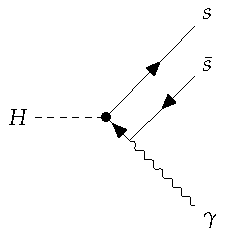
\includegraphics[height=0.27\mylength]{resources/H_rare_decays_vertices/v1.pdf}
            \setlength{\unitlength}{0.27\mylength}
            \caption{\footnotesize (a)}
    \end{subfigure}%
    \begin{subfigure}[t]{0.5\mylength}
            \centering
            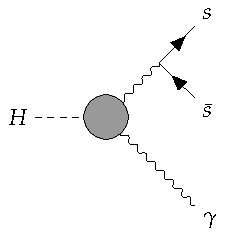
\includegraphics[height=0.27\mylength]{resources/H_rare_decays_vertices/v2.pdf}
            \setlength{\unitlength}{0.27\mylength}
            \caption{\footnotesize (b)}
    \end{subfigure}%
    \vspace*{-0.0cm}
    \caption{Direct and indirect contributions involved in the decays under analysis.}
    \label{fig:veritces}
    \vspace*{-0.0cm}
\end{figure}

\todo{unmeasured sectors of the higgs}

\todo{Explain how deviations from SM predictions in these sectors could point to new physics and justify the need for precise measurements.}

\comm{I don't know if I should add something else to this chapter? I have still some points to develope further, this is the first draft and like so is very provisional.}
